% !TeX root = er.tex

\chapter{Robots and Their Applications}\label{ch.basic}

\abstract*{This chapter starts with an overview and classification of robots: industrial robots, autonomous mobile robots, humanoid robots and educational robots. A specification is given of a generic educational robot used throughout the book: a small mobile robot with differential drive and horizontal and ground proximity sensors. A pseudocode is defined so that algorithms can be presented in a platform-independent manner. The chapter concludes with a detailed overview of the contents of the book.}

Although everyone seems to know what a robot is, it is hard to give a precise definition. The Oxford English Dictionary gives the following definition: ``A machine capable of carrying out a complex series of actions automatically, especially one programmable by a computer.'' This definition includes some interesting elements:
\begin{itemize}
\item ``Carrying out actions automatically.'' This is a key element in robotics, but also in many other simpler machines called automata. The difference between a robot and a simple automaton like a dishwasher is in the definition of what a ``complex series of actions'' is. Is washing clothes composed of a complex series of actions or not? Is flying a plane on autopilot a complex action? Is cooking bread complex? For all these tasks there are machines that are at the boundary between automata and robots.
\item ``Programmable by a computer'' is another key element of a robot, because some automata are programmed mechanically and are not very flexible. On the other hand computers are found everywhere, so it is hard to use this criterion to distinguish a robot from another machine.
\end{itemize}
A crucial element of robots that is not mentioned explicitly in the definition is the use of sensors. Most automata do not have sensors and cannot adapt their actions to their environment. Sensors are what enable a robot to carry out complex tasks. 

In Sects.~\ref{s.classification}--\ref{s.educational} of this introductory chapter we give a short survey of different types of robots. Section~\ref{s.generic} describes the generic robot we use and Sect.~\ref{s.alg-formalism} presents the pseudocode used to formalize the algorithms. Section~\ref{s.overview} gives a detailed overview of the contents of the book.

\section{Classification of robots}\label{s.classification}

Robots can be classified according to the environment in which they operate (Fig.~\ref{fig.classification1}).\index{robot!classification} The most common distinction is between \emph{fixed} and \emph{mobile} robots. These two types of robots have very different working environments and therefore require very different capabilities. Fixed robots are mostly industrial robotic manipulators that work in well defined environments adapted for robots. Industrial robots perform specific repetitive tasks such soldering or painting parts in car manufacturing plants. With the improvement of sensors and devices for human-robot interaction, robotic manipulators are increasingly used in less controlled environment such as high-precision surgery.

\begin{figure}
\begin{center}
% Classification of robots according to environment
\begin{tikzpicture}[node distance = 4mm and 1cm]
\node (robot) { \textsf{robot} };
\node (fixed) [below right=of robot] { \textsf{fixed} };
\node (mobile) [above right=of robot] { \textsf{mobile} };
\node (water) [above right=of mobile] { \textsf{aquatic} };
\node (land) [right=of mobile] { \textsf{terrestrial} };
\node (air) [below right=of mobile] { \textsf{airborne} };
\node (wheeled) [above right=of land] { \textsf{wheeled} };
\node (legged) [below right=of land] { \textsf{legged} };
\draw (robot) -- (fixed);
\draw (robot) -- (mobile);
\draw (mobile) -- (water);
\draw (mobile) -- (land);
\draw (mobile) -- (air);
\draw (land) -- (wheeled);
\draw (land) -- (legged);
\end{tikzpicture}
\end{center}
\caption{Classification of robots by environment and mechanism of interaction}\label{fig.classification1}
\end{figure}

By contrast, mobile robots are expected to move around and perform tasks in large, ill-defined and uncertain environments that are not designed specifically for robots. They need to deal with situations that are not precisely known in advance and that change over time. Such environments can include unpredictable entities like humans and animals. Examples of mobile robots are robotic vacuum cleaners and self-driving cars. 

There is no clear dividing line between the tasks carried out by fixed robots and mobile robots---humans may interact with industrial robots and mobile robots can be constrained to move on tracks---but it is convenient to consider the two classes as fundamentally different. In particular, fixed robots are attached to a stable mount on the ground, so they can compute their position based on their internal state, while mobile robots need to rely on their perception of the environment in order to compute their location.

There are three main environments\index{robot!environments} for mobile robots that require significantly different design principles because they differ in the mechanism of motion: aquatic (underwater exploration), terrestrial (cars) and aerial (drones). Again, the classification is not strict, for example, there are amphibious robots that move in both water and on the ground. Robots for these three environments can be further divided into subclasses: terrestrial robots can have legs or wheels or tracks, and aerial robots can be lighter-than-air balloons or heavier-than-air aircraft, which are in turn divided into fixed-wing and rotary-wing (helicopters).

\begin{figure}
\begin{center}
% Classification of robots according to task
\begin{tikzpicture}[node distance = 6mm and 1cm]
\node[text width=8mm,align=left] (robot) { \textsf{robot} };
\node[text width=12mm,align=left] (industrial) [above right=of robot] { \textsf{industrial} };
\node[text width=12mm,align=left] (service) [below right=of robot] {\textsf{service}};
\node[text width=20mm,align=left] (logistics) [above right=of industrial] { \textsf{logistics} };
\node[text width=20mm,align=left] (manufacturing) [below=of logistics] { \textsf{manufacturing} };
\node[text width=20mm,align=left] (medical) [below=of manufacturing] { \textsf{medical} };
\node[text width=20mm,align=left] (home) [below=of medical] { \textsf{home} };
\node[text width=20mm,align=left] (education) [below=of home] { \textsf{educational} };
\node[text width=20mm,align=left] (military) [below=of education] {  \textsf{defense}};
%
\draw (robot.north east) -- (industrial.south west);
\draw (robot.south east) -- (service.north west);
\draw (industrial.north east) -- (logistics.south west);
\draw (industrial.east) -- (manufacturing.west);
\draw (service.north east) -- (medical.south west);
\draw (service.east) -- (home.west);
\draw (service.south east) -- (education.north west);
\draw (service.south east |- 0,-15mm) -- (military.north west);
\end{tikzpicture}
\end{center}
\caption{Classification of robots by application field}\label{fig.classification2}
\end{figure}

Robots can be classified by intended application field and the tasks they perform (Fig.~\ref{fig.classification2}). We mentioned industrial robots which work in well-defined environments on production tasks. The first robots were industrial robots because the well-defined environment simplified their design.  Service robots, on the other hand, assist humans in their tasks. These include chores at home like vacuum clears, transportation like self-driving cars, and defense applications such as reconnaissance drones. Medicine, too, has seen increasing use of robots in surgery, rehabilitation and training. These are recent applications that require improved sensors and a closer interaction with the user.

\section{Industrial robots}\index{robot!industrial}

The first robots were industrial robots which replaced human workers performing simple repetitive tasks . Factory assembly lines can operate without the presence of humans, in a well-defined environment where the robot has to perform tasks in a specified order, acting on objects precisely placed in front of it (Fig.~\ref{fig.assemblyline}). 

\begin{figure}
\begin{center}
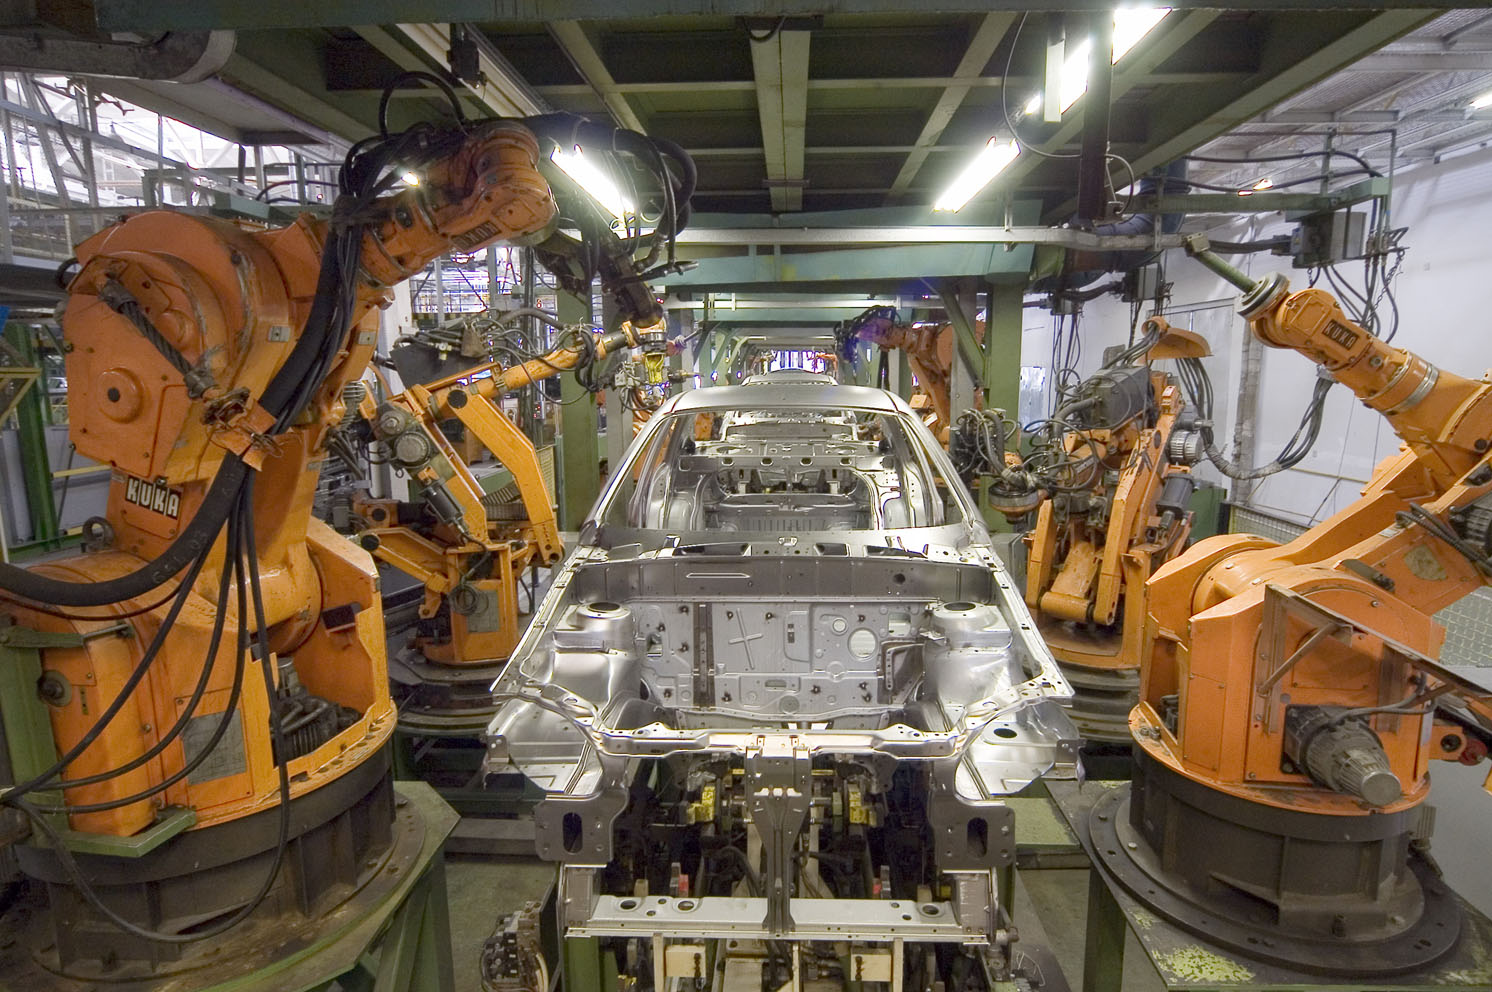
\includegraphics[width=\textwidth]{KUKA_Industrial_Robots_IR_wikimedia.jpg}
\end{center}
\caption{Robots on an assembly line in a car factory. Source: https://commons.wikimedia.org/wiki/File:AKUKA\_Industrial\_Robots\_IR.jpg by Mixabest (Own work). CC BY-SA 3.0 (http://creativecommons.org/licenses/by-sa/3.0) or GFDL (http://www.gnu.org/copyleft/fdl.html), via Wikimedia Commons.}\label{fig.assemblyline}
\end{figure}

One could argue that these are really automata and not robots. However, today's automata often rely on sensors to the extent that they can be considered as robots. However, their design is simplified because they work in a customized environment which humans are not allowed to access while the robot is working.

However, today's robots need more flexibility, for example, the ability to manipulate objects in different orientations or to recognize different objects that need to be packaged in the right order. The robot can be required to transport goods to and from warehouses. This brings additional autonomy, but the basic characteristic remains: the environment is more-or-less constrained and can be adapted to the robot.

Additional flexibility is required when industrial robots interact with humans and this introduces strong safety requirements, both for robotic arms and for mobile robots. In particular, the speed of the robot must be reduced and the mechanical design must ensure that moving parts are not a danger to the user. The advantage of humans working with robots is that each can perform what they do best: the robots perform repetitive or dangerous tasks, while humans perform more complex steps and define the overall tasks of the robot, since they are quick to recognize errors and opportunities for optimization.

\section{Autonomous mobile robots}
\index{robot!mobile}

Many mobile robots are remotely controlled, performing tasks such as pipe inspection, aerial photography and bomb disposal that rely on an operator controlling the device. These robots are not autonomous; they use their sensors to give their operator remote access to dangerous, distant or inaccessible places. Some of them can be semi-autonomous, performing subtasks automatically. The autopilot of a drone stabilizes the flight while the human chooses the flight path. A robot in a pipe can control its movement inside the pipe while the human searches for defects that need to be repaired. Fully \emph{autonomous mobile robots} do not rely on an operator, but instead they make decisions on their own and perform tasks, such as transporting material while navigating in uncertain terrain (walls and doors within buildings, intersections on streets) and in a constantly changing environment (people walking around, cars moving on the streets).

The first mobile robots were designed for simple environments, for example, robots that cleaned swimming pools or robotic lawn mowers. Currently, robotic vacuum cleaners are widely available, because it has proved feasible to build reasonably priced robots that can navigate an indoor environment cluttered with obstacles.

Many autonomous mobile robots are designed to support professionals working in structured environments such as warehouses. An interesting example is a robot for weeding fields (Fig.~\ref{fig.agri_robot}). This environment is partially structured, but advanced sensing is required to perform the tasks of identifying and removing weeds. Even in very structured factories, robot share the environment with humans and therefore their sensing must be extremely reliable.

\begin{figure}
\begin{center}
\includegraphics[width=0.8\textwidth]{ecorobotix.jpg}
\end{center}
\caption{Autonomous mobile robot weeding a field (Courtesy of Ecorobotix)}\label{fig.agri_robot}
\end{figure}

Perhaps the autonomous mobile robot getting the most publicity these days is the self-driving car. These are extremely difficult to develop because of the highly complex uncertain environment of motorized traffic and the strict safety requirements.

An even more difficult and dangerous environment is space. The Sojourner and Curiosity Mars rovers are semi-autonomous mobile robots. The Sojourner was active for three months in 1997. The Curiosity has been active since landing on Mars in 2012! While a human driver on Earth controls the missions (the routes to drive and the scientific experiments to be conducted), the rovers do have the capability of autonomous hazard avoidance.

Much of the research and development in robotics today is focused on making robots more autonomous by improving sensors and enabling more intelligent control of the robot. Better sensors can perceive the details of more complex situations, but to handle these situations, control of the behavior of the robot must be very flexible and adaptable. Vision, in particular, is a very active field of research because cameras are cheap and the information they can acquire is very rich. Efforts are being made to make systems more flexible, so that they can learn from a human or adapt to new situations. Another active field of research addresses the interaction between humans and robots. This involves both sensing and intelligence, but it must also take into account the psychology and sociology of the interactions.

\section{Humanoid robots}\index{robot!humanoid}

Science fiction and mass media like to represent robots in a humanoid form. We are all familiar with R2-D2 and 3-CPO, the robotic characters in the \emph{Star Wars} movies, but the concept goes far back. In the eighteenth century, a group of Swiss watchmakers---Pierre and Henri-Louis Jaquet-Droz and Jean-Fr\'{e}d\'{e}ric Leschot---built humanoid automata to demonstrate their mechanical skills and advertise their watches. Many companies today build humanoid robots for similar reasons.

Humanoid robots are a form of autonomous mobile robot with an extremely complex mechanical design for moving the arms and for locomotion by the legs. Humanoid robots are used for research into the mechanics of walking and into human-machine interaction. Humanoid robots have been proposed for performing services and maintenance in a house or a space station. They are being considered for providing care to the elderly who might feel anxious in the presence of a machine that did not appear human. On the other hand, robots that look very similar to humans can generate repulsion, a phenomenon referred to as the \emph{uncanny valley}.

Humanoid robots can be very difficult to design and control. They are expensive to build with multiple joints that can move in many different ways. Robots that use wheels or tracks are preferred for most applications because they are simpler, less expensive and robust.

\section{Educational robots}\label{s.educational}
\index{robot!educational}

Advances in the electronics and mechanics have made it possible to construct robots that are relatively inexpensive. Educational robots are used extensively in schools, both in classrooms and in extracurricular activities. The large number of educational robots makes it impossible to give a complete overview. Here we give few examples that are representative of robots commonly used in education.

\medskip

\noindent\textbf{Pre-assembled mobile robots}

Many educational robots are designed as pre-assembled mobile robots. Fig.~\ref{fig.thymio} shows the Thymio robot from Mobsya and Fig.~\ref{fig.dash} shows the Dash robot from Wonder Workshop. These robots are relatively inexpensive, robust and contain a large number of sensors and output components such as lights. An important advantage of these robots is that you can implement robotic algorithms ``out of the box,'' without investing hours in mechanical design and construction. However, pre-assembled robots cannot be modified, though many do support building extensions using, for example, \lego{} components.

\begin{figure}
\subfigures
\begin{minipage}{\textwidth}
\leftfigure{
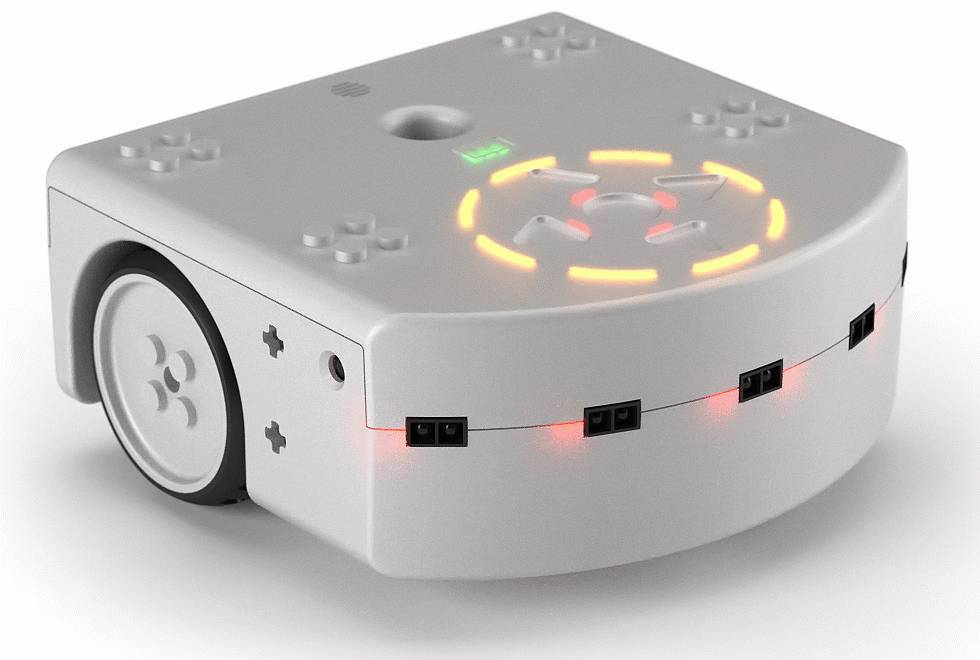
\includegraphics[width=.45\textwidth]{thymio}
}
\hspace{\fill}
\rightfigure{
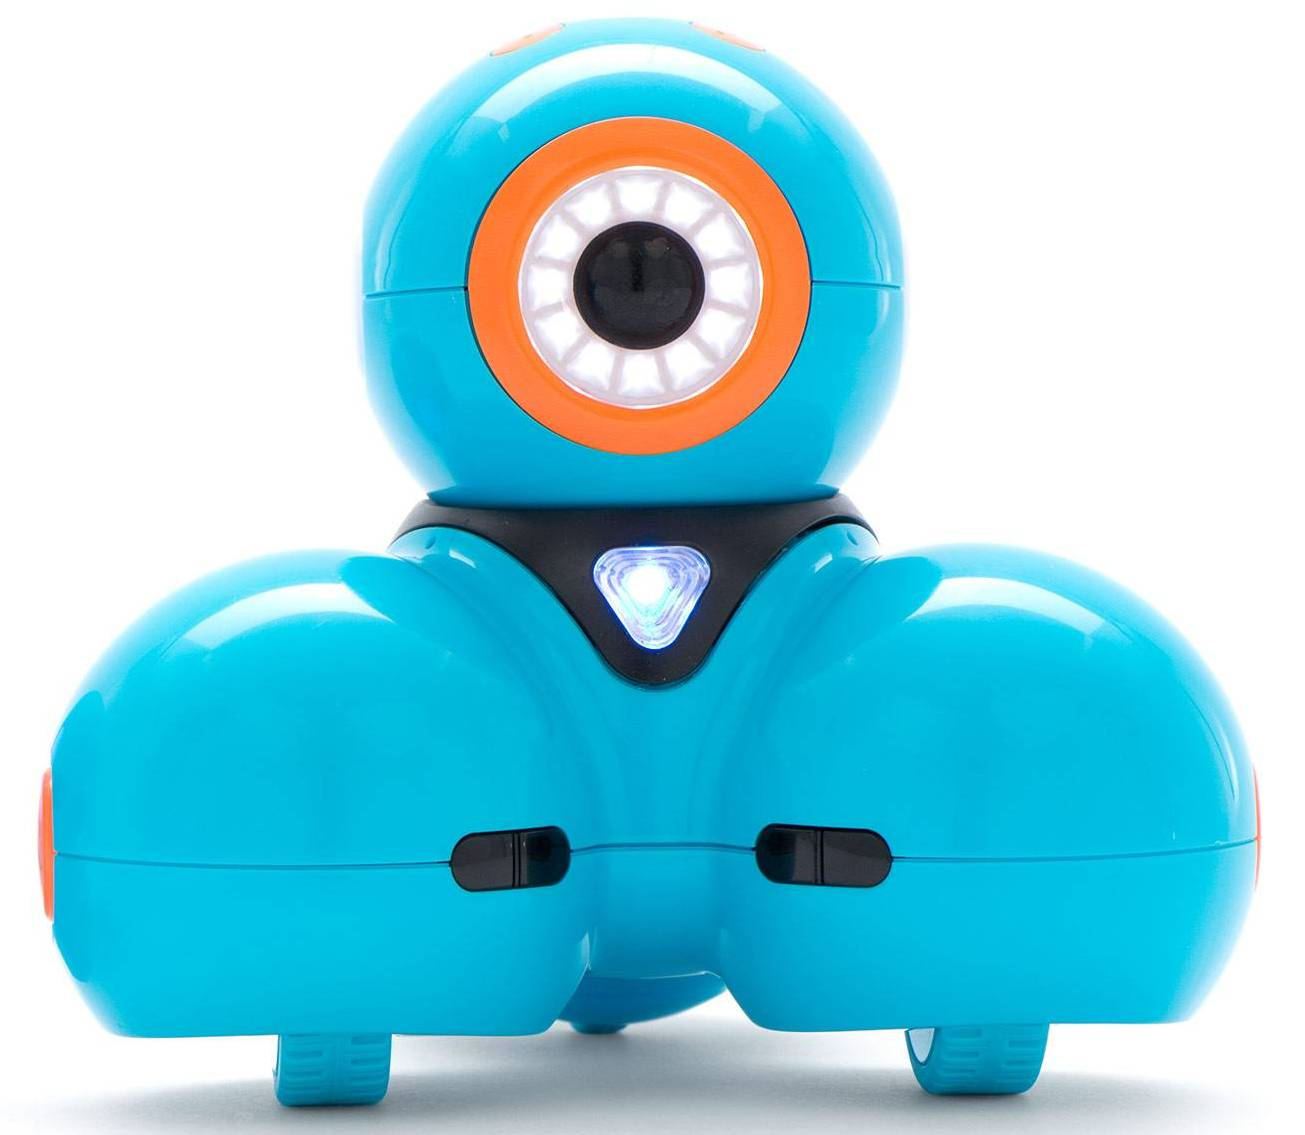
\includegraphics[width=.45\textwidth]{dash}
}
\leftcaption{Thymio robot. Source: https://www.thymio.org/en:mediakit by permission of \'{E}cole Polytechnique F\'{e}d\'{e}rale de Lausanne and \'{E}cole Cantonale d'Art de Lausanne.}\label{fig.thymio}
\rightcaption{Dash robot. Source: https://www.makewonder.com/mediakit by permission of Wonder Workshop.}\label{fig.dash}
\end{minipage}
\end{figure}

\medskip

\noindent\textbf{Robotics kits}

The \lego{} Mindstorms robotics kits (Fig.~\ref{fig.lego}) were introduced in 1998.\footnote{The figure shows the latest version called \emph{EV3} introduced in 2014.} A kit consists of standard \lego{} bricks and other building components, together with motors and sensors, and a programmable brick which contains the computer that controls the components of the robot. The advantage of robotics kits is that they are flexible: you can design and build a robot to perform a specific task, limited only by your imagination. A robotics kit can also be used to teach students mechanical design. The disadvantages of robotics kits are that they are more expensive than simple pre-assembled robots and that exploration of robotics algorithms depends on the one's ability to successfully implement a robust mechanical design.

A recent trend is to replace fixed collections of bricks by parts constructed by 3D printers. An example is the Poppy Ergo Jr robotic arm (Fig.~\ref{fig.poppy}). The use of 3D printed parts allows more flexibility in the creation of the mechanical structure and greater robustness, but does require access to a 3D printer. 

\begin{figure}
\subfigures
\begin{minipage}{\textwidth}
\leftfigure{
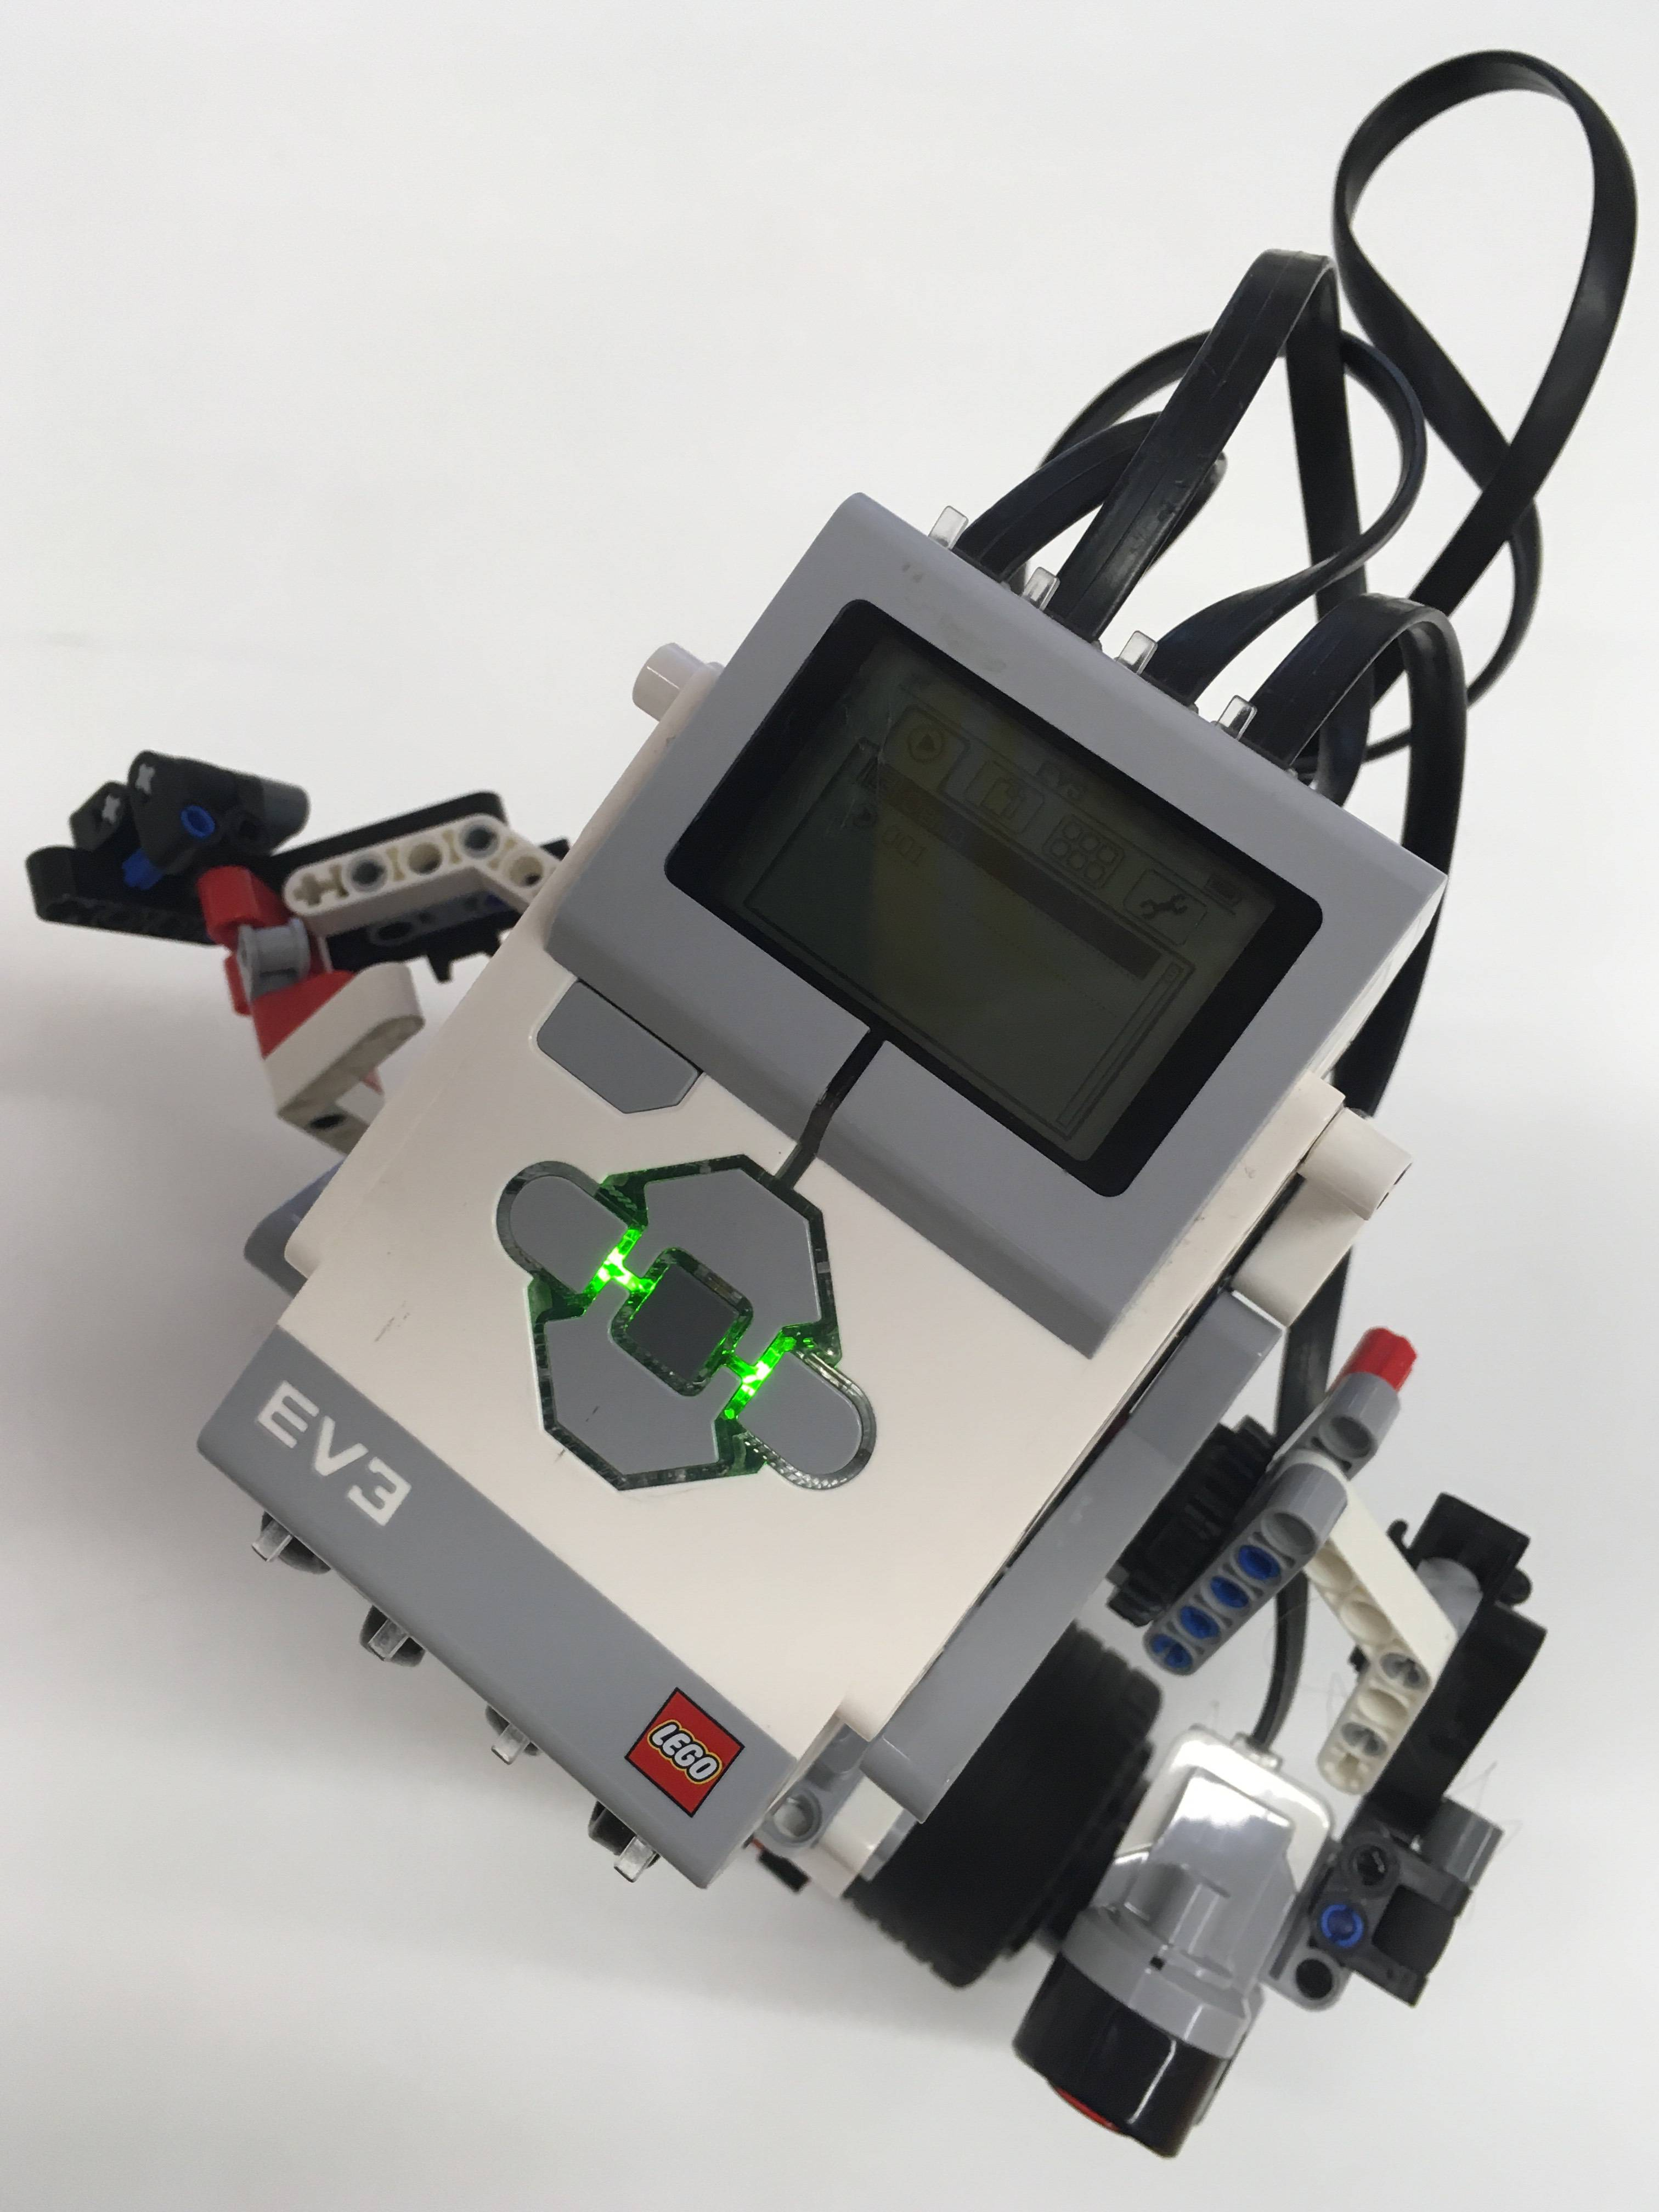
\includegraphics[width=.4\textwidth]{lego}
}
\hspace{\fill}
\rightfigure{
\hspace*{-8mm}\includegraphics[width=.55\textwidth]{ErgoJr.jpg}
}
\end{minipage}
\leftcaption{\lego{} Mindstorms EV3 (Courtesy of Adi Shmorak, Intelitek)}\label{fig.lego}
\rightcaption{Poppy Ergo Jr robotic arms (Courtesy of the Poppy Project)}\label{fig.poppy}
\end{figure}

\medskip

\noindent\textbf{Robotic arms}

To act on its environment, the robot needs an \emph{actuator} which is a component of a robot that affects the environment. Many robots, in particular robotic arms used in industry, affect the environment through \emph{end effectors}, usually grippers or similar tools (Figs.~\ref{fig.assemblyline}, \ref{fig.sortballs}, \ref{fig.robots-pulling}). The actuators of mobile robots are the motors that cause the robot to move, as well as components such as the vacuum pump of a vacuum cleaner.

Educational robots are usually mobile robots whose only actuators are its motors and display devices such as lights, sounds or a screen. End effectors can be built with robotics kits or by using additional components with pre-assembled robots, although educational robotic arms do exist (Fig.~\ref{fig.poppy}). Manipulation of objects introduces complexity into the design; however, since the algorithms for end effectors are similar to the algorithms for simple mobile robots, most of the activities in the book will assume only that your robot has motors and display devices.

\medskip

\noindent\textbf{Software development environments}

Every educational robotics system includes a \emph{software development environment}\index{software development environment}. The programming language can be a version of a standard programming language like Java or Python. Programming is simplified if a block-based language is used, usually a language based upon Scratch or Blockly (Fig.~\ref{fig.ide-blocks}).

\begin{figure}
\begin{center}
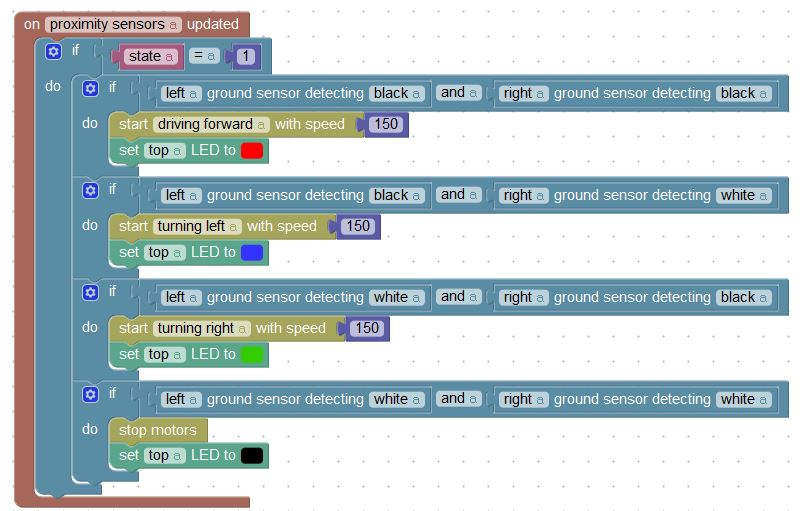
\includegraphics[width=.7\textwidth]{blockly}
\end{center}
\caption{Blockly software for the Thymio robot}\label{fig.ide-blocks}
\end{figure}

To further simplify programming a robot by young students, a fully graphical programming notation can be used. Figures~\ref{fig.ide-thymio} shows VPL (Visual Programming Language), a graphical software environment for the Thymio robot. It uses event-action pairs: when the event represented by the block on the left occurs, the actions in the following blocks are performed.

\begin{figure}
\begin{center}
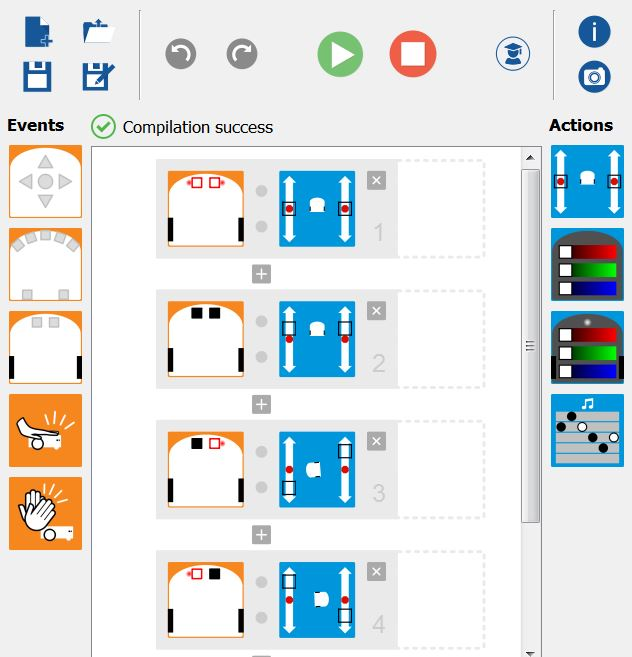
\includegraphics[width=.7\textwidth]{vpl}
\end{center}
\caption{VPL software for the Thymio robot}\label{fig.ide-thymio}
\end{figure}

Figure~\ref{fig.ide-dash} shows the graphical software environment for the Dash robot. It also uses events and actions, where the actions are represented by nodes and events are represented by arrows between nodes.

\begin{figure}
\begin{center}
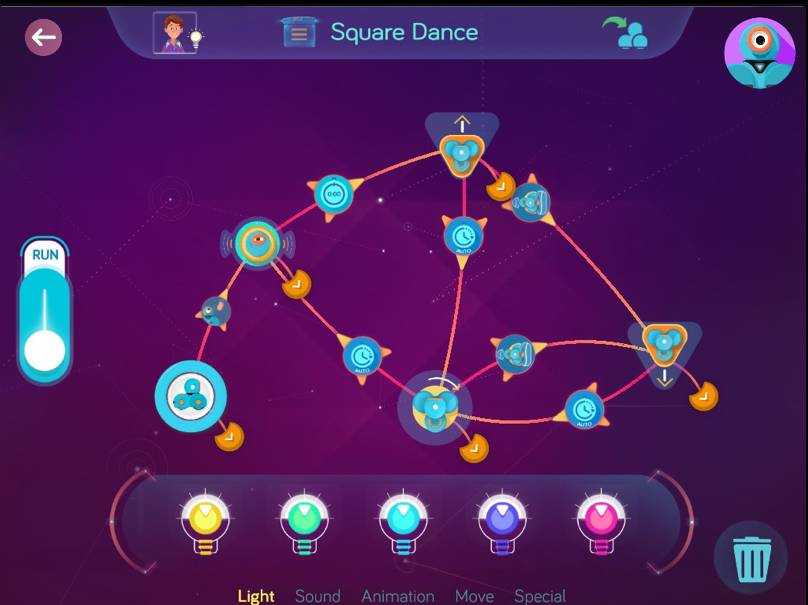
\includegraphics[width=.8\textwidth]{wonder}
\end{center}
\caption{Wonder software for the Dash robot (Courtesy of Wonder Workshop)}\label{fig.ide-dash}
\end{figure}

\section{The Generic Robot}\label{s.generic}

\index{robot!generic}
This section presents the description of a generic robot that we use to present the robotics algorithms. The capabilities of the generic robot are similar to those found in educational robots, but the one you use may not have all the capabilities assumed in the presentations so you will have to improvise. You may not understand all the terms in the following description just yet, but it is important that the specification be formalized. Further details will be given in later chapters.

\subsection{Differential drive}

The robot is a small autonomous vehicle with \emph{differential drive},\index{differential drive} meaning that it has two wheels that are driven by independent motors (Fig.~\ref{fig.differential}). To cause the robot to move, set the motor power to a value from $-100$ (full power backwards) through $0$ (stopped) to $100$ (full power forwards). There is no predefined relationship between the motor power and the velocity of robot. The motor can be connected to the wheels through different gear ratios, the type of tires on the wheels affects their traction, and sandy or muddy terrain can cause the wheels to slip.

\begin{figure}
\begin{center}
\begin{tikzpicture}[scale=1.2]
\pic[scale=1.5] at (0,0) { robot };
\draw[densely dotted,thick] (12mm,0) circle[radius=6pt];
\draw[->] (16mm,10mm) node[right] {\p{support (on the bottom of the robot)}} -- (13mm,3mm);
\draw[->,thick] (20mm,0) -- node[below] {\p{forward} } +(18mm,0);
\draw[raxis] (0,0) -- (0,15mm);
\draw[raxis] (0,0) -- (0,-15mm);
\draw[raxis] (0,0) -- (11pt,0);
\draw[raxis] (0,0) -- (-11pt,0);
\end{tikzpicture}
\end{center}
\caption{Robot with differential drive\label{fig.differential}}
\end{figure}

Figure~\ref{fig.differential} shows a view of the robot from above. The front of the robot is the curve to the right which is also the forward direction of the robot's motion. The wheels (black rectangles) are on the left and right sides of the rear of the robot's body. The dot is the point on the axle halfway between the wheels. When the robot turns, it turns around an axis vertical to this point. For stability, towards the front of the robot there is a support or non-driven wheel.

\begin{quote}
\begin{center}
\textbf{Mechanical drawing}
\end{center}
A broken line is the standard notation in mechanical engineering for the \emph{axis of symmetry} in a component such as a wheel. When the side view of a wheel is displayed, the intersection of the two axes of symmetry denotes the axis of rotation that is perpendicular to the plane of the page. To avoid cluttering the diagrams, we simplify the notation by only showing broken lines for an \emph{axis of rotation} of a component such as a wheel. In addition, the intersection denoting a perpendicular axis is usually abbreviated to a cross, possibly contained within the wheel or its axle.
\end{quote}

Differential drive has several advantages: it is simple since it has only two motors without additional components for steering  and it allows the robot to turn in place. In a car, two wheels are driven together (or four wheels are driven in pairs) and there is a separate complex mechanism for steering called \emph{Ackermann steering}\index{Ackermann steering}. Since a car cannot turn in place, drivers must perform complicated maneuvers such as parallel parking; human drivers readily learn to do this, but such maneuvers are difficult for an autonomous system. An autonomous robot needs to perform intricate maneuvers with very simple movements, which is why differential drive is the preferred configuration: it can easily turn to any heading and then move in that direction.

The main disadvantage of a differential drive system is that it requires a third point of contact with the ground unlike a car which already has four wheels to support it and thus can move easily on difficult terrain. Another disadvantage is that it cannot drive laterally without turning. There are configurations that enable a robot to move laterally (Sect.~\ref{s.holonomic}), but they are complex and expensive. Differential drive is also used in tracked vehicles such as earth-moving equipment and military tanks. These vehicles can maneuver in extremely rough terrain, but the tracks produce a lot of friction so movement is slow and not precise.

\begin{quote}
\begin{center}
\textbf{Setting power or setting speed}
\end{center}
The power supplied by a motor is regulated by a \emph{throttle}, such as a pedal in a car or levers in an airplane or boat. Electrical motors used in mobile robots are controlled by modifying the voltage applied to the motors using a technique called \emph{pulse width modulation}. In many educational robots, control algorithms such as those described in Chap.~\ref{ch.control}, are used to ensure that the motors rotate at a specified \emph{target speed}. Since we are interested in concepts and algorithms for designing robots, we will express algorithms in terms of supplying power and deal separately with controlling speed.
\end{quote}


\subsection{Proximity sensors}

The robot has \emph{horizontal proximity sensors}\index{sensor!proximity} that can detect an object near the robot. There exist many technologies that can be used to construct these sensors, such as infrared, laser, ultrasound; the generic robot represents robots that use any of these technologies. We do specify that the sensors have the following capabilities: A horizontal proximity sensor can measure the distance (in centimeters) from the robot to an object and the angle (in degrees) between the front of the robot and the object. Figure~\ref{fig.generic-sensor} shows an object located at $3\,$ cm from the center of the robot at an angle of $45^{\circ}$ from the direction in which the robot is pointing.\footnote{See Appendix~\ref{ch.units} on the conventions for measuring angles.}

\begin{figure}
\subfigures
\leftfigure{
\begin{tikzpicture}
\pic[scale=1.2] at (0,0) { robot };
\draw[->] (0,0) -- node[sloped,above] {$3\,$cm} (45:2.5cm) node[above right=-4pt] {$\bullet$};
\draw[dashed] (0,0) node[above,xshift=20pt] {$45^{\circ}$}-- (2.5,0);
\draw (10pt,0) arc [start angle=0, end angle=45, radius=10pt];
\fill[gray] (0,0) circle[radius=4pt];
\end{tikzpicture}
}
\hspace{\fill}
\rightfigure{
\begin{tikzpicture}
\pic[scale=1.2] at (0,0) { robot2 };
\end{tikzpicture}
}
\leftcaption{Robot with a rotating sensor (gray dot)\label{fig.generic-sensor}}
\rightcaption{Robot with two ground sensors on the bottom of the robot (gray rectangles)}\label{fig.generic-ground}
\end{figure}

In practice, an educational robot will have a small number of sensors, so it may not be able detect objects in all directions. Furthermore, inexpensive sensors will not be able to detect objects that are far away and their measurements will not be accurate. The measurements will also be affected by environmental factors such as the type the object, the ambient light, and so on. To simplify our algorithms, we do not assume any predefined limitations, but when you implement the algorithms you will have to take the limitations into account.

\subsection{Ground sensors}

\emph{Ground sensors}\index{sensor!ground} are mounted on the bottom of the robot. Since these sensors are very close to the ground, there is no meaning to distance or angle; instead, the sensor measures the brightness of the light reflected from the ground in arbitrary values between $0$ (totally dark) and $100$ (totally light). The generic robot has two ground sensors mounted towards the front of the robot (Fig.~\ref{fig.generic-ground}), though sometimes we present algorithms that use only one sensor. The figure shows a top view of the robot although the ground sensors are on the \emph{bottom} of the robot.

\subsection{Embedded computer}\label{s.embedded}

The robot is equipped with an \emph{embedded computer} (Fig.~\ref{fig.computer}). The precise specification of the computer is not important but we do assume certain capabilities. The computer can read the values of the sensors and set the power of the motors. There is a way of displaying information on a small screen or using colored lights. Signals and data can be input to the computer using buttons, a keypad or a remote control.

\begin{figure}
\begin{center}
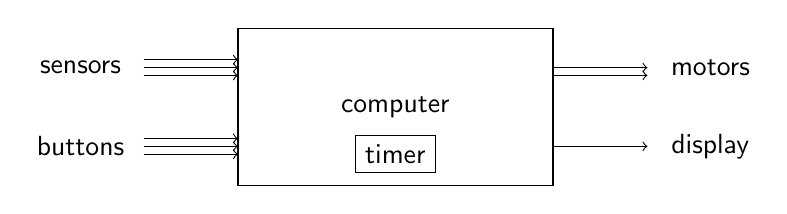
\begin{tikzpicture}
\node[draw,rectangle,minimum width=4cm,minimum height=2cm] at (0,0) {\textsf{computer}};
\node[draw,rectangle] at (0,-.6) {\textsf{timer}};
\node at (-4,.5) {\textsf{sensors}};
\node at (-4,-.5) {\textsf{buttons}};
\draw[->] (-3.2,.4) -- (-2,.4);
\draw[->] (-3.2,.5) -- (-2,.5);
\draw[->] (-3.2,.6) -- (-2,.6);
\draw[->] (-3.2,-.4) -- (-2,-.4);
\draw[->] (-3.2,-.5) -- (-2,-.5);
\draw[->] (-3.2,-.6) -- (-2,-.6);
\node at (4,.5) {\textsf{motors}};
\node at (4,-.5) {\textsf{display}};
\draw[->] (2,.4) -- (3.2,.4);
\draw[->] (2,.5) -- (3.2,.5);
\draw[->] (2,-.5) -- (3.2,-.5);
\end{tikzpicture}
\caption{Embedded computer}\label{fig.computer}
\end{center}
\end{figure}

Data is input to the computer by \emph{events} such as touching a button. The occurrence of an event causes a procedure called an \emph{event handler}\index{event handler} to be run. The event can be detected by the hardware, in which case the term \emph{interrupt} is used, or it can be detected by the software, usually, by \emph{polling}, where the operating system checks for events at predefined intervals. When the event handler terminates, the previous computation is started up again.

Event handlers are different from sequential programs that have an initial instruction that inputs data and a final instruction that displays the output, because event handlers are run in response to unpredictable events. Event handling is used to implement graphic user interfaces on computers and smartphones: when you click on or touch an icon an event handler is run. On a robot, an event can be a discrete input like touching a key. Events can also occur when a continuous value like the value read by a sensor goes above or below a predefined value called a \emph{threshold}\index{threshold}.

The computer includes a \emph{timer}\index{timer} which functions like a stopwatch on a smartphone. A timer is a variable that is \emph{set} to a period of time, for example, $0.5$ second, which is represented as an integer number milliseconds or microseconds ($0.5$ second is $500$ milliseconds). The hardware clock of the computer causes an interrupt at fixed intervals and the operating system decrements the value of the timer. When its value goes to zero, we say that the timer has \emph{expired}; an interrupt occurs.

Timers are used to implement repeated events like flashing a light on and off. They are also used for \emph{polling}\index{polling}, an alternative to event handlers: instead of performing a computation when an event occurs, sensors are read and stored periodically. More precisely, polling occurs as an event handler when a timer expires, but the design of software using polling can be quite different from the design of event-based software.

\section{The algorithmic formalism}\label{s.alg-formalism}

Algorithms that are implemented as computer programs are used by the embedded computer to control the behavior of the robot. We do not give programs in any specific programming language; instead, algorithms are presented in \emph{pseudocode},\index{pseudocode} a structured format using a combination of natural language, mathematics and programming structures. Algorithm~\ref{alg.integer-mult} is a simple algorithm for integer multiplication using repeated addition. The input of the algorithm is a pair of integers and the output is the product of the two input values. The algorithm declares three integer variables \p{x}, \p{a}, \p{b}. There are five statements in the executable part. Indentation is used (as in the Python programming language) to indicate the scope of the loop. An arrow is used for assignment so that the familiar symbols $=$ and $\neq$ can be used for equality and inequality in mathematical formulas.\footnote{Many programming languages use \texttt{=} for assignment and then \texttt{==} for equality and \texttt{!=} for inequality. This is confusing because equality $x=y$ is symmetrical, but assignment is not \texttt{x=x+1}. We prefer to retain the mathematical notation.}

\begin{figure}
\begin{alg}{Integer multiplication}{integer-mult}           
&\idv{}integer x \ass 0&\\
&\idv{}integer a, b&\\
\hline
\stl{}&a \ass input an integer&\\
\stl{}&b \ass input a non-negative integer&\\
\stl{}&while b $\neq$ 0&\\
\stl{}&\idc{} x \ass x $+$ a&// Add the value a to x\\
\stl{}&\idc{} b \ass b $-$ 1&// \ \ for each b\\
\end{alg}
\end{figure}

The motor power is set using assignment statements:
\begin{quote}
\p{left-motor-power} \ass $50$\\
\p{right-motor-power} \ass $-50$
\end{quote}

We have defined our proximity sensors as returning the distance to a detected object and its angle relative to the forward direction of the robot, but it will often be more convenient to use natural language expressions such as:
\begin{quote}
\p{when object detected in front}\\
\p{when object not detected in back}
\end{quote}

\section{An overview of the content of the book}\label{s.overview}

The first six chapters form the core of robotics concepts and algorithms.
\begin{description}
\item [\textbf{Chapter \ref{ch.basic} Robots and Their Applications}] This chapter surveys and classifies robots. It also specifies the generic robot and formalisms used to present algorithms in this book.
\smallskip
\item [\textbf{Chapter \ref{ch.sensors} Sensors}] Robots are more than remotely controlled appliances like a television set. They show autonomous behavior based on detecting objects in their environment using sensors. This chapter gives an overview of the sensors used by robots and explains the concepts of range, resolution, precision and accuracy. It also discusses the nonlinearity of sensors and how to deal with it.
\smallskip
\item [\textbf{Chapter \ref{ch.reactive} Reactive Behavior}] When an autonomous robot detects an object in its environment, it reacts by changing its behavior. This chapter introduces robotics algorithms where the robot directly changes its behavior based upon input from its sensors. Braitenberg vehicles are simple yet elegant examples of reactive behavior. The chapter presents several variants of line following algorithms.
\smallskip
\item [\textbf{Chapter \ref{ch.fmg} Finite State Machines}] A robot can be in different states, where its reaction to input from its sensors depends not only on these values but also on the current state. Finite state machines are a formalism for describing states and the transitions between them that depend on the occurrence of events.
\smallskip
\item [\textbf{Chapter \ref{ch.motion} Robotic Motion and Odometry}] Autonomous robots explore their environment, performing actions. Hardly a day goes by without a report on experience with self-driving cars. This chapter reviews concepts related to motion (distance, time, velocity, acceleration), and then presents odometry, the fundamental method that a robot uses to move from one position to another. Odometry is subject to significant errors and it is important to understand their nature.

The second part of the chapter gives an overview of advanced concepts of robotic motion: wheel encoders and inertial navigation systems that can improve the accuracy of odometry, and degrees of freedom and holonomy that affect the planning of robotic motion.
\smallskip
\item [\textbf{Chapter \ref{ch.control} Control}] An autonomous robot is a closed loop control system because input from its sensors affects its behavior which in turn affects what is measured by the sensors. For example, a self-driving car approaching a traffic light can brake harder as it gets close to the light. This chapter describes the mathematics of control systems that ensure optimal behavior: the car actually does stop at the light and the braking is gradual and smooth.
\end{description}

An autonomous mobile robot must somehow navigate from a start position to a goal position, for example, to bring medications from the pharmacy in a hospital to the patient. Navigation is a fundamental problem in robotics that is difficult to solve. The following four chapters present navigation algorithms in various contexts.
\begin{description}
\item [\textbf{Chapter \ref{ch.obstacle} Local Navigation: Obstacle Avoidance}] The most basic requirement from a mobile robot is that it does not crash into walls, people and other obstacles. This is called \emph{local} navigation because it deals with the immediate vicinity of the robot and not with goals that the robot is trying to reach. The chapter starts with wall following algorithms that enable a robot to move around an obstacle; these algorithms are similar to algorithms for navigating a maze. The chapter describes a probabilistic algorithm that simulates the navigation by a colony of ants searching for a food source.
\smallskip
\item [\textbf{Chapter \ref{ch.local} Localization}] Once upon a time before every smartphone included GPS navigation, we used to navigate with maps printed on paper. A difficult problem is localization: can you determine your current position on the map? Mobile robots must solve the same localization problem, often without the benefit of vision. The chapter describes localization by trigonometric calculations from known positions. This is followed by sections on probabilistic localization: A robot can detect a landmark but there may be many similar landmarks on the map. By assigning probabilities and updating them as the robot moves through the environment, it can eventually determine its position with relative certainty.
\smallskip
\item [\textbf{Chapter \ref{ch.mapping} Mapping}] But where does the map come from? Accurate street maps are readily available, but a robotic vacuum cleaner does not have a map of your apartment. An undersea robot is used to explore an unknown environment. To perform localization the robot needs a map, but to create a map of an unknown environment the robot needs to localize itself, in the sense that it has to know how far it has moved from one point of the environment to another. The solution is to perform simultaneous localization and mapping. The first part of the chapter describes an algorithm for exploring an environment to determine the locations of obstacles. Then an simplified algorithm for simultaneous localization and mapping is presented.
\smallskip
\item [\textbf{Chapter \ref{ch.map-based} Mapping-Based Navigation}] Now that the robot has a map, suppose that it is assigned a task that requires it to move from a start position to a goal position. What route should it take? This chapter presents two algorithms for path planning: Dijkstra's algorithm, a classic algorithm for finding the shortest path in a graph, and the \astar{} algorithm, a more efficient version of Dijkstra's algorithm that uses heuristic information.
\end{description}

The following chapters present advanced topics in robotics. They are independent of each other so you can select which ones to study and in what order.
\begin{description}
\item [\textbf{Chapter \ref{ch.fuzzy} Fuzzy Logic Control}] Control algorithms (Chap.~\ref{ch.control}) require the specification of a precise target value: a heating system needs the target temperature of a room and a cruise control system needs the target speed of a car. An alternate approach called fuzzy logic uses imprecise specifications like cold, cool, warm, hot, or very slow, slow, fast, very fast. This chapter presents fuzzy logic and shows how it can be used to control a robot approaching an object.
\smallskip
\item [\textbf{Chapter \ref{ch.image} Image Processing}] Most robotic sensors measure distances and angles using lasers, sound or infrared light. We humans rely primarily on our vision. High quality digital cameras are inexpensive and found on every smartphone. The difficulty is to process and interpret the images taken by the camera, something our brains do instantly. Digital image processing has been the subject of extensive research and its algorithms are used in advanced robots that can afford the needed computing power. In this chapter we survey image processing algorithms and show how an educational robot can demonstrate the algorithms even without a camera.
\smallskip
\item [\textbf{Chapter \ref{ch.neural} Neural Networks}] Autonomous robots in highly complex environments cannot have algorithms for every possible situation. A self-driving car cannot possibly know in advance all the different vehicles and configurations of vehicles that it encounters on the road. Autonomous robots must learn from their experience and this is a fundamental topic in artificial intelligence that has been studied for many years. This chapter presents one approach to learning: artificial neural networks modeled on the neurons in our brains. A neural network uses learning algorithms to modify its internal parameters so that it continually adapts to new situations that it encounters.
\smallskip
\item [\textbf{Chapter \ref{ch.machine} Machine Learning}] Another approach to learning is a statistical technique called machine learning. This chapter describes two algorithms for distinguishing between two alternatives, for example, distinguishing between a traffic light that is red and one that is green. The first algorithm, called linear discriminant analysis, is based on the means and variances of a set of samples. The second algorithm uses perceptrons, a form of neural network that can distinguish between alternatives even when the samples do not satisfy the statistical assumptions needed for linear discriminant analysis.
\smallskip
\item [\textbf{Chapter \ref{ch.swarm} Swarm Robotics}] If you need to improve the performance of a system, it is often easier to use multiple instances of a component rather than trying to improve the performance of an individual component. Consider a problem such as surveying an area to measure the levels of pollution. You can use a single very fast (and expensive) robot, but it can be easier to use multiple robots, each of which measures the pollution in a small area. This is called swarm robotics by analogy with a swarm of insects that can find the best path between their nest and a source of food. The fundamental problem in swarm robotics, as in all concurrent systems, is to develop methods for coordination and communications among the robots. This chapter presents two such techniques: exchange of information and physical interactions.
\smallskip
\item [\textbf{Chapter \ref{ch.kinematics} Kinematics of a Robotic Manipulator}] Educational robots are small mobile robots that move on a two-dimensional surface. There are mobile robots that move in three-dimensions: robotic aircraft and submarines. The mathematics and algorithms for three-dimensional motion were developed in another central field of robotics: manipulators that are used extensively in manufacturing. This chapter presents a simplified treatment of the fundamental concepts of robotic manipulators (forward and inverse kinematics, rotations, homogeneous transforms) in two dimensions, as well as a taste of three-dimensional rotations.
\end{description}

There are two appendices:
\begin{description}
\item [\textbf{Appendix \ref{ch.units} Units of Measurement}] This appendix contains Table A.1 with units of measurements. Table A.2 gives prefixes that are used with these units.
\smallskip
\item [\textbf{Appendix \ref{ch.math} Mathematical derivations and tutorials}] This chapter contains tutorials that review some of the mathematical concepts used in the book. In addition, some of the detailed mathematical derivations have been collected here so as not to break the flow of the text.
\end{description}

\section{Summary}

Robots are found everywhere: in factories, homes and hospitals, and even in outer space. Much research and development is being invested in developing robots that interact with humans directly. Robots are used in schools in order to increase students' motivation to study STEM and as a pedagogical tool to teach STEM in a concrete environment. The focus of this book is the use of educational robots to learn robotic algorithms and to explore their behavior.

Most educational robots have a similar design: a small mobile robot using differential drive and proximity sensors. To make this book platform-independent, we defined a generic robot with these properties. The algorithms presented in this book for the generic robot should be easy to implement on educational robots, although different robots will have different capabilities in terms of the performance of their motors and sensors. The algorithms are presented in a language-independent pseudocode that should be easy to translate into any textual or graphics language that your robot supports.

\section{Further reading}

For a non-technical overview of robotics with an emphasis on biologically-inspired and humanoid robotics, see Winfield~\cite{vsi}.

The International Organization for Standardization (ISO)\footnote{No, this is not a mistake! ISO is the official abbreviated name of the organization and not an acronym in any of its three official languages: English, French and Russian.} publishes standards for robotics. On their website \url{https://www.iso.org/} you can find the catalog of robotics (ISO/TC 299) and formal definitions of robotics concepts: ISO 8373:2012 Robots and robotic devices---Vocabulary and ISO 19649:2017 Mobile robots---Vocabulary.

The topics in this book are presented in greater detail in advanced textbooks on robotics such as \cite{dudek,siegwart}. Their introductory chapters give many examples of robots.

Educational robots come with documentation of their capabilities and software development environments. There are also textbooks based upon specific robots, for example, \cite{trobaugh} on programming the \lego{} Mindstorms robotics kits and \cite{kumar} on using Python to program the Scribbler robots. The design of the Visual Programming Language (VPL) is presented in \cite{shin2014idc}.

Pseudocode is frequently used in textbooks on data structures and algorithms, starting from the classic textbook \cite{aho}. The style used here is taken from \cite{pcdp2}.

\bibliographystyle{spmpsci}
\bibliography{er}
